\documentclass{article}
\usepackage[utf8]{inputenc}
\usepackage{booktabs}
\usepackage{graphicx}
\usepackage{geometry}
\geometry{margin=1.8cm}
\begin{document}
\title{Quant Research Report}
\author{Cursor + Grok Bot}
\date{\today}
\maketitle

\section{Metryki strategii (SMA 20/50)}
\begin{table}[h]
\centering
\small
\begin{tabular}{lrrrrrrrr}
\toprule
Ticker & Ann Vol & Sharpe & Max Dd & Beta & Total Return & Win Rate & Avg Win & Avg Loss \\
\midrule
SPY & 12.08\% & 0.78 & -28.89\% & 0.37 & 79.93\% & 39.10\% & 0.66\% & -0.68\% \\
QQQ & 16.18\% & 0.79 & -26.52\% & 0.43 & 117.75\% & 37.11\% & 0.91\% & -0.98\% \\
TLT & 10.80\% & 0.10 & -16.27\% & -0.07 & 3.78\% & 19.99\% & 0.79\% & -0.75\% \\
\bottomrule
\end{tabular}
\end{table}

\section{Equity Curve}
\begin{figure}[h]
\centering
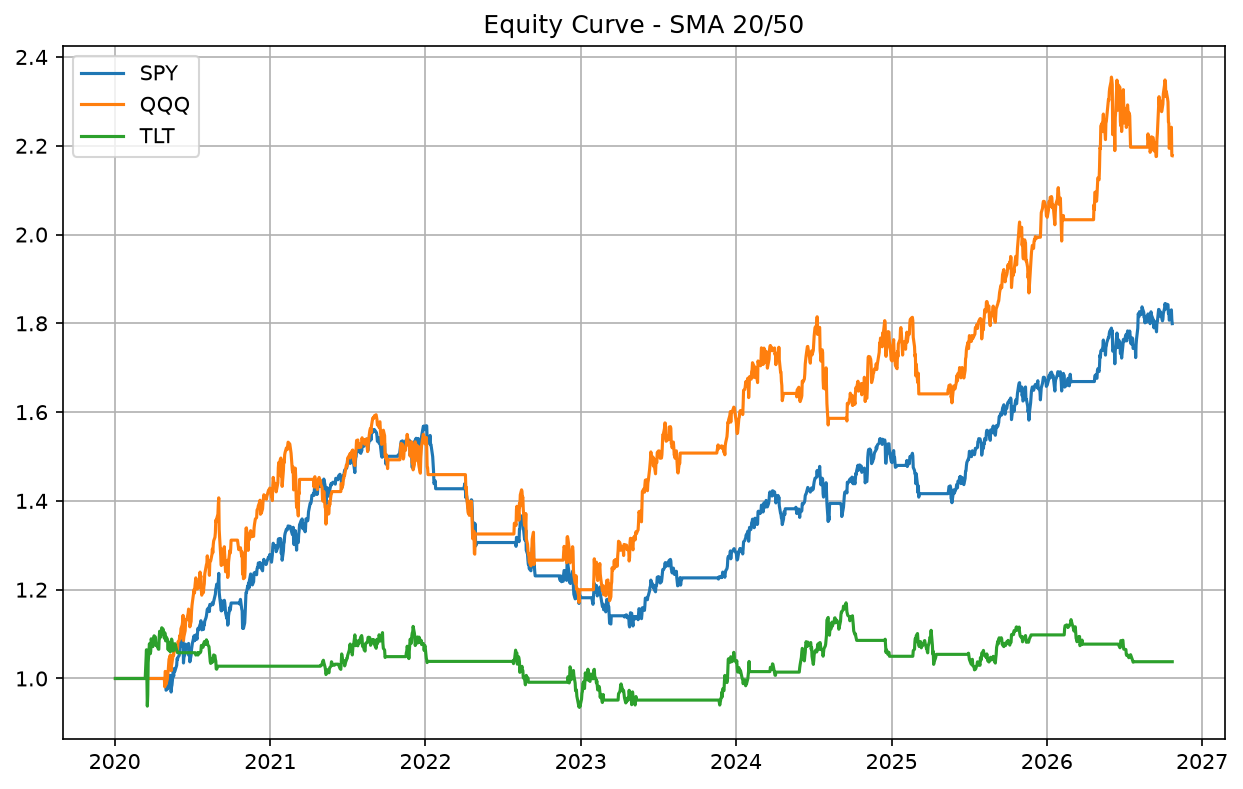
\includegraphics[width=0.95\textwidth]{equity_curve.png}
\caption{Equity Curve strategii SMA 20/50}
\end{figure}

\end{document}
